\documentclass[10pt]{article}

\usepackage[margin=0.82in]{geometry}
\usepackage[T1]{fontenc}
\usepackage{lmodern}
\usepackage{microtype}
\usepackage{amsmath,amssymb,amsthm,mathtools}
\usepackage{booktabs}
\usepackage{enumitem}
\usepackage{xcolor}
\usepackage{tikz}
\usepackage[hidelinks]{hyperref}

\usetikzlibrary{arrows.meta,positioning}
\setlist{nosep,leftmargin=*}
\setlength{\parindent}{1.05em}
\setlength{\parskip}{0.12em}
\setlength{\emergencystretch}{2em}
\numberwithin{equation}{section}

\newtheorem{theorem}{Theorem}[section]
\newtheorem{corollary}[theorem]{Corollary}
\newtheorem{lemma}[theorem]{Lemma}
\theoremstyle{definition}
\newtheorem{definition}[theorem]{Definition}
\theoremstyle{remark}
\newtheorem{remark}[theorem]{Remark}

\newcommand{\C}{\mathbb C}
\newcommand{\R}{\mathbb R}
\newcommand{\N}{\mathbb N}
\newcommand{\ee}{\mathrm e}
\newcommand{\ip}[2]{\langle #1,#2\rangle}
\newcommand{\norm}[1]{\lVert #1\rVert}

\title{\bfseries Energy sets how far a quantum future can be hidden}
\author{Michael Haufschild}
\date{July 28, 2026}

\begin{document}
\maketitle

\begin{abstract}
How much dynamical resource is required to conceal a different future beyond
an observed part of a quantum system?  We establish a necessary-and-sufficient
scaling law.  For arbitrary bounded generators on arbitrary complete complex
normed state spaces, agreement of the first \(N\) coefficients seen by any
continuous scalar probe forces a dimension-free exact-tail bound on every
later response.  At generator action \(u=\norm{z}\Lambda\le N/\ee\), every
response gap is at most \(4\norm{\ell}\norm{x}/\sqrt{2\pi N}\); a gap that
remains nonzero therefore eventually requires \(u>N/\ee\).  The law remains
valid with an arbitrary finite profile of measured coefficient errors, whose
complete contribution is explicit.  For self-adjoint nearest-neighbour
quantum chains, an observed radius \(R\) fixes \(N=2R+3\) return
coefficients.  If a fixed return-probability gap survives for increasing
\(R\), then eventually
\[
 \Lambda_R T>\frac{2R+3}{\ee}.
\]
The order is exact.  For every target time, every strictly earlier
observation window and every positive accuracy, one finite constant \(a\)
works at every radius: an isospectral nearest-neighbour family with
\[
 \Lambda_R T\le \frac{\pi}{2}(4R+2a+5)
\]
has one exactly common local Hamiltonian record, indistinguishable earlier
return records, and target-time return probabilities filling the complete
interval \([0,1]\).  Thus the energy--time cost of hiding a quantum future
beyond distance \(R\) is \(\Theta(R)\).  The lower law covers finite and
bounded infinite-dimensional, unitary and non-unitary dynamics; the upper
law is attained by an explicit one-dimensional Hermitian chain.  This turns
quantum extrapolation from a qualitative impossibility into a universal
resource law.
\end{abstract}

\noindent\textbf{One-sentence summary.}
To hide a fixed change in a quantum future beyond \(R\) observed layers,
energy times time must grow linearly with \(R\), and linear growth is enough
to hide every possible return probability.

\section{The prediction problem}

Quantum speed limits ask how quickly a known system can move between states
\cite{MandelstamTamm1945,MargolusLevitin1998,NessEtAl2022}.  We ask the
inverse question: how much energy--time capacity must an incompletely known
system possess for two locally identical descriptions to produce different
later observations?

The distinction matters whenever an observer knows a local Hamiltonian
neighbourhood and a finite dynamical record but not the complete generator.
Hamiltonian learning, recurrence measurements and the certification of
quantum simulators all have this form
\cite{BaireyAradLindner2019,RauerEtAl2018}.  Locality alone suggests a
causal cone \cite{LiebRobinson1972}; energy bounds alone constrain motion.
Neither statement identifies the resource required to keep an alternative
future outside an observed region.

Recent quantum-extrapolation results show that finite records can contain
``fog banks'' of complete future unpredictability
\cite{ManosWeilenmannNavascues2026}.  That establishes a broad
ill-posedness phenomenon.  The question answered here is sharper:
\begin{quote}
\emph{What is the least asymptotic energy--time scaling that permits a
nonvanishing hidden future beyond an increasing exact record?}
\end{quote}
The answer is linear.  It is necessary for every bounded generator and
sufficient in an explicitly local Hermitian quantum system.

\begin{figure}[t]
\centering
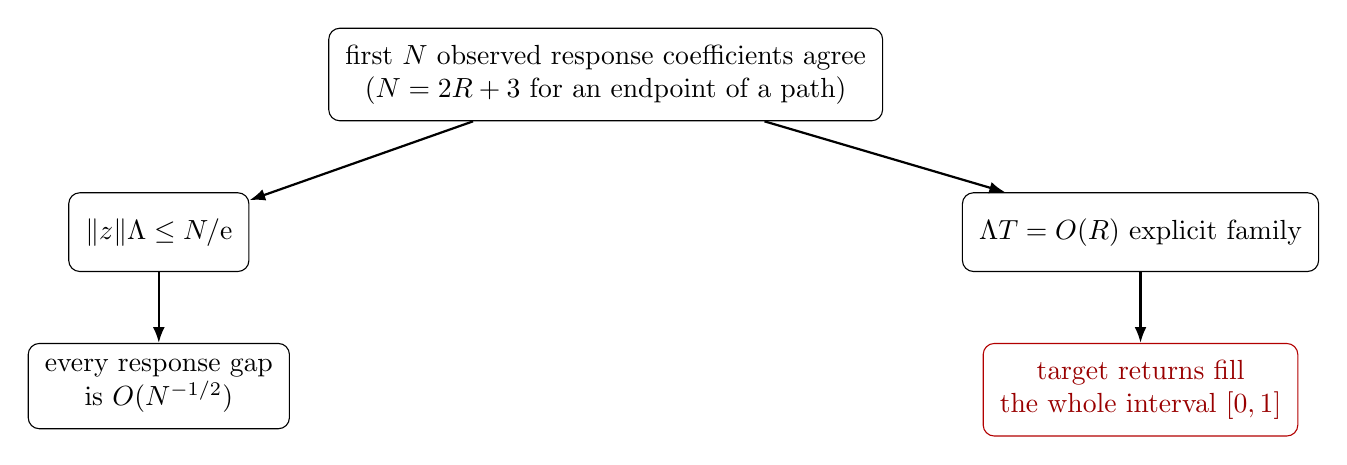
\begin{tikzpicture}[
  node distance=9mm and 10mm,
  box/.style={draw,rounded corners,align=center,inner sep=6pt,
    minimum height=10mm},
  arr/.style={-{Latex[length=2mm]},thick}
]
\node[box] (record) {first \(N\) observed response coefficients agree\\
  (\(N=2R+3\) for an endpoint of a path)};
\node[box,below left=of record] (sub) {
  \(\norm{z}\Lambda\le N/\ee\)};
\node[box,below right=of record] (lin) {
  \(\Lambda T=O(R)\) explicit family};
\node[box,below=of sub] (fade) {every response gap\\
  is \(O(N^{-1/2})\)};
\node[box,below=of lin,draw=red!70!black,text=red!60!black]
  (complete) {target returns fill\\the whole interval \([0,1]\)};
\draw[arr] (record) -- (sub);
\draw[arr] (record) -- (lin);
\draw[arr] (sub) -- (fade);
\draw[arr] (lin) -- (complete);
\end{tikzpicture}
\caption{\textbf{Linear hidden-future law.}
At the universal \(N/\ee\) action boundary, common observed coefficients
force a vanishing future discrepancy.  A one-dimensional quantum chain
attains complete target ambiguity with only linear energy--time growth.}
\label{fig:law}
\end{figure}

\section{A causal law for every bounded generator}

Let \(X\) be any complete complex normed vector space, let
\(G,K:X\to X\) be bounded linear generators, let \(x\in X\), and let
\(\ell:X\to\C\) be any continuous linear probe.  Define the entire response
\begin{equation}
 F_G(z)=\ell(\ee^{zG}x),\qquad z\in\C .
\label{eq:response}
\end{equation}
No inner product, finite dimension, self-adjointness, normality, positivity
or unitarity is assumed.

\begin{theorem}[Universal scalar-record causal horizon]
\label{thm:universal}
Suppose
\[
 \norm{G},\norm{K}\le\Lambda,\qquad
 \ell(G^m x)=\ell(K^m x)\quad(0\le m<N).
\]
Put \(u=\norm{z}\Lambda\).  Then, for every \(z\in\C\),
\begin{equation}
 |F_G(z)-F_K(z)|
 \le
 2\norm{\ell}\norm{x}
 \left(\ee^u-\sum_{m=0}^{N-1}\frac{u^m}{m!}\right).
\label{eq:exact-tail}
\end{equation}
If \(N>0\) and \(u\le N/\ee\), then
\begin{equation}
 |F_G(z)-F_K(z)|
 \le
 \frac{4\norm{\ell}\norm{x}}{\sqrt{2\pi N}}.
\label{eq:critical}
\end{equation}
Consequently, along every sequence with \(N\to\infty\), a response
difference bounded below by one fixed positive number eventually requires
\begin{equation}
 \norm{z}\Lambda>\frac{N}{\ee}.
\label{eq:universal-critical}
\end{equation}

More generally, if the measured coefficients obey arbitrary error budgets
\[
 |\ell(G^m x)-\ell(K^m x)|\le\eta_m,\qquad 0\le m<N,
\]
then the right side of Eq.~\eqref{eq:exact-tail} is augmented by exactly
\begin{equation}
 \mathcal E_N(z)=
 \sum_{m=0}^{N-1}\frac{\norm{z}^m}{m!}\eta_m.
\label{eq:calibration}
\end{equation}
At \(u\le N/\ee\), the response gap is therefore at most
\(\mathcal E_N(z)+4\norm{\ell}\norm{x}/\sqrt{2\pi N}\).
\end{theorem}

\begin{proof}
The response has the absolutely convergent expansion
\[
 F_G(z)=\sum_{m=0}^{\infty}
   \frac{z^m}{m!}\ell(G^m x).
\]
The first \(N\) terms cancel.  Submultiplicativity gives
\[
 \big|\ell(G^m x)-\ell(K^m x)\big|
 \le 2\norm{\ell}\norm{x}\Lambda^m,
\]
and summing the uncancelled terms gives Eq.~\eqref{eq:exact-tail}.

If \(u\le N/\ee\), consecutive terms in the exact tail have ratio
\[
 \frac{u}{N+j+1}\le\frac{N}{\ee(N+1)}<\frac12.
\]
The complete tail is therefore at most twice its first term.  The global
Stirling bound
\[
 N!\ge\sqrt{2\pi N}\left(\frac{N}{\ee}\right)^N
\]
then proves Eq.~\eqref{eq:critical}.  Its right side vanishes, proving
Eq.~\eqref{eq:universal-critical}.  Without exact cancellation, retain the
first \(N\) terms and apply their individual error budgets; this gives
Eq.~\eqref{eq:calibration}, while the unobserved tail is unchanged.
\end{proof}

The theorem is a law about observed response data, not hidden state
equality.  Only the scalar coefficients accessible to \(\ell\) must agree.
It applies without change to bounded infinite-dimensional operators.  Every
finite-dimensional linear evolution is also included, so Hamiltonian,
non-Hermitian effective and vectorized dissipative generators obey the same
factorial horizon whenever the stated response coefficients and generator
norm are controlled.  Open-system speed limits constrain state motion
\cite{DelCampoEtAl2013}; calibration-aware limits profile nuisance
parameters \cite{WaniAlKuwari2026}.  Theorem~\ref{thm:universal} instead
controls continuation from an arbitrary approximate scalar response jet,
with every calibration contribution retained.

\section{Local quantum chains turn coefficient order into distance}

Let \(\mathcal H_n=\C^{n+1}\) with path basis
\(e_0,\ldots,e_n\).  A path Hamiltonian is a self-adjoint tridiagonal
operator \(J\).  The endpoint return amplitude and probability are
\begin{equation}
 A_J(t)=\ip{e_0}{\ee^{itJ}e_0},
 \qquad
 P_J(t)=|A_J(t)|^2.
\label{eq:return}
\end{equation}
Two path Hamiltonians are \(R\)-locally equal if their onsite terms through
site \(R\) and their bonds through \(R\leftrightarrow R+1\) are identical.
Energy zero is a gauge for return probabilities.  We call \(\Lambda\) a
common centred bandwidth radius for \(J,K\) if there is a real \(c\) such
that
\begin{equation}
 \norm{J-cI},\norm{K-cI}\le\Lambda .
\label{eq:centered-radius}
\end{equation}
This definition is invariant under a common shift of both Hamiltonians.

\begin{lemma}[Exact round-trip record]
\label{lem:roundtrip}
If \(J\) and \(K\) are \(R\)-locally equal, then
\begin{equation}
 \ip{e_0}{J^m e_0}=\ip{e_0}{K^m e_0},
 \qquad 0\le m\le2R+2.
\label{eq:moments}
\end{equation}
\end{lemma}

\begin{proof}
After at most \(R+1\) nearest-neighbour steps, an endpoint vector cannot
leave sites \(0,\ldots,R+1\), so
\(J^a e_0=K^a e_0\) for \(a\le R+1\).
Self-adjointness splits every endpoint moment of order \(a+b\) into
\[
 \ip{e_0}{J^{a+b}e_0}
 =\ip{J^a e_0}{J^b e_0}.
\]
Choosing \(a,b\le R+1\) proves Eq.~\eqref{eq:moments}.
\end{proof}

The factor \(2R+2\) is the round trip to the first unobserved bond and back.
It converts the universal coefficient index into a spatial distance without
a thermodynamic or continuum approximation.

\begin{theorem}[Dimension-free local quantum causal bound]
\label{thm:local-bound}
Let \(J,K\) be arbitrary finite self-adjoint nearest-neighbour path
Hamiltonians that are \(R\)-locally equal.  If \(\Lambda\) is a common
centred bandwidth radius, then for every \(t\in\R\),
\begin{equation}
 |P_J(t)-P_K(t)|
 \le
 4\ee^{\Lambda|t|}
 \frac{(\Lambda|t|)^{2R+3}}{(2R+3)!}.
\label{eq:prob-bound}
\end{equation}
At the linear action boundary
\(\Lambda|t|\le(2R+3)/\ee\), the sharper exact-tail estimate is
\begin{equation}
 |P_J(t)-P_K(t)|
 \le
 \frac{8}{\sqrt{2\pi(2R+3)}}.
\label{eq:prob-critical}
\end{equation}
The bound contains no Hilbert-space dimension.
\end{theorem}

Apply Theorem~\ref{thm:universal} after the common energy-origin shift and
use \(N=2R+3\).  Both displayed bounds follow from the corresponding
factorial and exact-tail response estimates.  The probability statement uses
\(\big||a|^2-|b|^2\big|\le2|a-b|\) for unitary return amplitudes.

\begin{corollary}[Linear energy--distance necessity]
\label{cor:necessity}
For every sequence of such pairs \(J_R,K_R\), suppose
\[
 \norm{J_R-c_RI},\norm{K_R-c_RI}\le\Lambda_R,\qquad
 |P_{J_R}(T)-P_{K_R}(T)|\ge\varepsilon>0
\]
for some real \(c_R\) at every \(R\).  Then eventually
\begin{equation}
 \Lambda_R|T|>\frac{2R+3}{\ee}.
\label{eq:necessity}
\end{equation}
\end{corollary}

This is stronger than saying the energy scale must diverge.  It fixes its
minimum order: a future difference hidden beyond distance \(R\) consumes
energy times time at least linearly in \(R\).

\section{Linear energy is sufficient to hide every return}

The lower law would be only a speed limit without a matching process.  We
now show that the linear order is attained while holding fixed the physical
features most likely to leak the answer: preparation, measurement, complete
spectrum, local couplings and the full earlier return record.

\begin{definition}[Future-complete local record]
Fix \(T>0\), \(0\le H<T\), \(\delta>0\), radius \(R\) and centred norm
ceiling \(\Lambda\).  A baseline \(J_0\) has a future-complete local record
if there are a family \((J_p)_{p\in[0,1]}\) and one real energy origin \(c\)
such that all members
\begin{enumerate}
\item are self-adjoint nearest-neighbour Hamiltonians on one finite path;
\item have one common spectrum, including multiplicity;
\item use the same endpoint preparation \(e_0\) and return test;
\item are \(R\)-locally equal to \(J_0\);
\item satisfy
\[
 \sup_{|t|\le H}|P_{J_p}(t)-P_{J_0}(t)|<\delta;
\]
\item satisfy \(P_{J_p}(T)=p\) and
\(\norm{J_p-cI}\le\Lambda\).
\end{enumerate}
\end{definition}

\begin{theorem}[Linear achievability of the complete future]
\label{thm:achievability}
For every \(T>0\), \(0\le H<T\) and \(\delta>0\), there is
\(a\in\N\), depending only on \(H/T\) and \(\delta\), such that for every
\(R\) a future-complete local record exists with a path index \(n_R\) and
norm ceiling satisfying
\begin{equation}
 n_R\le4R+2a+5,\qquad
 \Lambda_R\le\frac{\pi(4R+2a+5)}{2T}.
\label{eq:upper}
\end{equation}
One dimension, spectrum and baseline work simultaneously for every
\(p\in[0,1]\) at that radius.
\end{theorem}

\subsection{Exact construction}

Choose an odd \(n=2q+1\) and the common energy lattice
\begin{equation}
 E_j=\frac{\pi j}{T},\qquad 0\le j\le n .
\label{eq:energies}
\end{equation}
Let
\[
 w_j=2^{-n}\binom nj
\]
and let \(v_j=w_j[1+(-1)^{n-j}]\), the normalized parity-conditioned
weights.  For \(p\in[0,1]\), set
\begin{equation}
 w_j^{(p)}=(1-\sqrt p)\,w_j+\sqrt p\,v_j .
\label{eq:weights}
\end{equation}
Finite-difference cancellation gives
\begin{equation}
 \sum_{j=0}^n w_j^{(p)}E_j^m
 =\sum_{j=0}^n w_jE_j^m,
 \qquad 0\le m<n .
\label{eq:moment-match}
\end{equation}
At the target time, the full binomial amplitude vanishes and the
parity-conditioned amplitude has unit modulus.  Therefore
\begin{equation}
 P_p(T)=p.
\label{eq:target}
\end{equation}

For \(|t|\le H\), the exact amplitude discrepancy is bounded by
\begin{equation}
 |A_p(t)-A_0(t)|
 \le
 \left|\sin\frac{\pi H}{2T}\right|^n .
\label{eq:window}
\end{equation}
Because \(H<T\), the sine factor is strictly below one.  A single additive
integer \(a=a(H/T,\delta)\) therefore makes the right-hand side small enough
for every required moment order.  Taking the moment order \(2R+2\) yields
\(q\le2R+2+a\) and hence \(n\le4R+2a+5\).

Finally, Gram--Schmidt orthogonalization of
\(1,E,\ldots,E^n\) in each weighted spectral measure produces its canonical
Jacobi matrix.  Multiplication by energy becomes a self-adjoint
nearest-neighbour Hamiltonian.  The common moments
\eqref{eq:moment-match} force its onsite and bond entries through radius
\(R\) to agree exactly, a finite inverse-Jacobi principle
\cite{GesztesySimon1997,SimonOPRL}.  All matrices are unitary conjugates of
the same diagonal energy operator, so their full spectra, including
multiplicity, coincide.  Since \(0\le E_j\le\pi n/T\), the common midpoint
choice \(c=\pi n/(2T)\) gives
\[
 \norm{J_p-cI}\le\frac{\pi n}{2T}.
\]
Return probabilities and local equality are unchanged by this energy-origin
shift, so Eq.~\eqref{eq:upper} follows.  This proves
Theorem~\ref{thm:achievability}.

The endpoint \(p=1\) has a sharp structural boundary.  Every \(p<1\) has
strictly positive spectral weights and a canonical path with every adjacent
bond nonzero.  At \(p=1\), the constructed path has one zero bond beyond the
common local prefix; moreover, every tridiagonal fixed-protocol realization
of that parity-supported endpoint must contain a zero bond.  Thus exact
perfect return is the only disconnected endpoint, whereas the complete open
interval of target probabilities is attained by connected chains.

The construction also has an exact many-body lift.  Second quantization of
every member gives a number-conserving free-fermion chain.  In every fixed
particle-number sector and for every \(p\), it has a complete Slater
eigenbasis with the same subset-sum energy list.  Thus isospectrality is not
confined to the one-excitation block: it persists sector by sector across
the full fermionic Fock construction.  The return protocol and the resource
\(\Lambda T\) remain the one-excitation endpoint experiment and its centred
one-particle bandwidth; no interacting-spectrum claim is made.

\section{The optimal law}

A future-complete record contains in particular a \(p=0\) model and a
\(p=1\) model, hence a unit target-time gap.  Corollary
\ref{cor:necessity} applies to every cofinal sequence of such records.
Theorems \ref{thm:local-bound} and \ref{thm:achievability} therefore give
\begin{equation}
 \boxed{
 \frac{2R+3}{\ee}
 < \Lambda_R T
 \quad\text{is necessary eventually},\qquad
 \Lambda_R T
 \le \frac{\pi}{2}(4R+2a+5)
 \quad\text{is sufficient}.
 }
\label{eq:optimal-law}
\end{equation}
For fixed earlier-window resolution, complete hidden-future capacity has
the exact asymptotic order
\begin{equation}
 \Lambda_R T=\Theta(R).
\label{eq:theta}
\end{equation}

This is the central result.  Increasing dimension is not the operative
escape: the lower bound is dimension-free.  Increasing record precision is
not the escape either: \(a\) is fixed once \(H/T\) and \(\delta\) are fixed,
and the radius cost remains linear.  The resource is the gauge-invariant
dimensionless centred Hamiltonian action \(\Lambda T\).  Restoring units
replaces it by
\(\Lambda T/\hbar\).

\section{Infinite systems and the bounded--unbounded boundary}

The lower half of the law already covers every bounded operator on every
complete complex normed state space, including infinite-dimensional spaces
and operators with continuous spectrum.  Thus no finite-dimensional
compactness is used in the causal direction.

There is also an exact unbounded infinite realization of the opposite
regime.  Lift each finite energy in Eq.~\eqref{eq:energies} to
\begin{equation}
 E_{j,k}=E_j+\frac{2\pi k}{T},\qquad
 \gamma_k=2^{-(k+1)},\qquad k\in\N .
\label{eq:ladder}
\end{equation}
Coordinate multiplication by \(E_{j,k}\) on its maximal square-summability
domain is self-adjoint and unbounded, and infinitely many distinct energy
levels are populated.  The return amplitude factorizes:
\begin{equation}
 A_p^\infty(t)=A_p(t)
 \sum_{k=0}^{\infty}\gamma_k
 \exp\!\left(\frac{2\pi i k t}{T}\right).
\label{eq:factor}
\end{equation}
The second factor has modulus at most one and equals one at \(T\).  It
therefore preserves every target probability and cannot enlarge any earlier
discrepancy.  Every finite moment block is preserved through a triangular
binomial decomposition, so every prescribed finite canonical Jacobi prefix
also survives.

The two infinite statements meet without contradiction.  A fixed bounded
infinite generator with all observed coefficients fixed obeys the causal
law.  A cofinal hidden-future sequence must drive its norm scale linearly to
infinity, and the exact infinite witness is correspondingly unbounded.
Unboundedness is therefore the resource predicted by Eq.~\eqref{eq:optimal-law},
not an artefact added after construction.

\section{Physical consequences}

\subsection{An inverse quantum speed limit}

Conventional speed limits bound the time required for one known state to
become distinguishable.  Equation~\eqref{eq:optimal-law} bounds the
energy--time required for two models with the same observed past to retain
a distinguishable future.  It is simultaneously:
\begin{enumerate}
\item a no-hiding law below the linear threshold;
\item a construction proving complete hiding at linear cost;
\item a certificate independent of unobserved Hilbert-space dimension.
\end{enumerate}
The matched lower and upper orders are what distinguish the result from a
Taylor estimate, a Lieb--Robinson upper cone or a qualitative
extrapolation obstruction.

\subsection{Closed, open and effective dynamics}

The sharp saturation uses ordinary Hermitian nearest-neighbour dynamics.
The causal theorem is broader.  It covers every bounded complex generator
and every continuous scalar response, including non-normal effective
matrices and finite-dimensional vectorized master-equation generators.
Neither complete positivity nor trace preservation is needed for the
mathematical bound; physical channels satisfying those properties form a
subclass.  The theorem therefore separates two ingredients often conflated
in forecasting: linear generator control creates the universal causal
horizon, while Hermitian spatial locality supplies an exact conversion
between coefficient order and distance.

\subsection{A direct falsification protocol}

The saturating matrices are one-particle tight-binding Hamiltonians and,
equivalently, one-excitation blocks of number-conserving nearest-neighbour
spin chains.  An experiment can:
\begin{enumerate}
\item calibrate the common onsite terms and bonds through radius \(R\);
\item independently bound a common centred Hamiltonian radius by
\(\Lambda\);
\item prepare and test the endpoint excitation;
\item compare target-time returns.
\end{enumerate}
Exact equality is not required for a response-jet test.  Let
\(\widetilde J=J-cI\), \(\widetilde K=K-cI\), \(N=2R+3\), and suppose the
measured centred endpoint moments have certified errors
\[
 \left|\ip{e_0}{\widetilde J^m e_0}
 -\ip{e_0}{\widetilde K^m e_0}\right|\le\eta_m
 \quad(0\le m<N).
\]
At \(\Lambda|t|\le N/\ee\), Theorem~\ref{thm:universal} gives the
operational probability budget
\begin{equation}
 |P_J(t)-P_K(t)|
 \le
 2\sum_{m=0}^{N-1}\frac{|t|^m}{m!}\eta_m
 \frac{8}{\sqrt{2\pi N}}.
\label{eq:noisy-protocol}
\end{equation}
Thus a violation of Eq.~\eqref{eq:prob-bound}, or of the error-aware
Eq.~\eqref{eq:noisy-protocol}, falsifies at least one certified premise.
Neither bound relies on a guessed dimension.  The family in
Theorem~\ref{thm:achievability} supplies exact target values for protocol
design.  Preparation, readout, leakage and decoherence may be added as
separately measured error terms; no device-feasibility claim is made.

\section{Relation to prior limits}

Lieb--Robinson theory bounds propagation under a known decomposition into
local interactions \cite{LiebRobinson1972}.  Quantum speed limits bound
state-space motion from energy information
\cite{MandelstamTamm1945,MargolusLevitin1998,NessEtAl2022}.
Universal scrambling limits constrain the earliest thermalization of
information from entropy and temperature data \cite{VikramShouGalitski2026}.
Inverse Jacobi theory reconstructs local tridiagonal coefficients from
spectral data \cite{GesztesySimon1997,SimonOPRL}.  Quantum fog-bank
constructions demonstrate that future statistics can become completely
unpredictable from finite data
\cite{ManosWeilenmannNavascues2026}.

The present result is not a new version of any one of these ingredients.
Its content is the matched quantifier structure:
\begin{enumerate}
\item every complete complex normed state space, every bounded pair of
generators and every continuous scalar probe obey one exact-tail horizon,
including arbitrary coefficient-error profiles;
\item every persistent response gap crosses the explicit \(N/\ee\) action
boundary;
\item every radius, strict earlier window, accuracy and target probability
is attained by one isospectral nearest-neighbour family;
\item the attaining norm grows only linearly, proving the lower order exact.
\end{enumerate}
The law answers a resource question left open by qualitative
unpredictability: it identifies how much dynamical capacity is necessary
and sufficient to hide the future.

\section{Scope of the conclusion}

Equation~\eqref{eq:optimal-law} is unconditional for the stated classes.
It does not assert indeterminism: every candidate Hamiltonian has perfectly
deterministic unitary evolution.  It does not assert superluminal signalling:
the hidden structure is outside the calibrated local record.  It does not
identify a cosmological, gravitational or thermodynamic arrow.  It does
answer the complete question posed here: for bounded linear response
dynamics, common finite response data enforce a factorial causal horizon;
for local quantum paths, the energy--time cost of retaining a fixed hidden
future beyond distance \(R\) is linear, and the same linear order already
permits every physically possible return probability.

\section*{Data availability}

No datasets were generated or analysed.  All constructions and estimates
needed to evaluate the results are given in the Article.

\section*{Competing interests}

The author declares no competing interests.

\begin{thebibliography}{99}

\bibitem{MandelstamTamm1945}
Mandelstam, L. \& Tamm, I.
The uncertainty relation between energy and time in non-relativistic
quantum mechanics.
\emph{J. Phys. USSR} \textbf{9}, 249--254 (1945).

\bibitem{MargolusLevitin1998}
Margolus, N. \& Levitin, L. B.
The maximum speed of dynamical evolution.
\emph{Physica D} \textbf{120}, 188--195
(1998). doi:10.1016/S0167-2789(98)00054-2.

\bibitem{NessEtAl2022}
Ness, G., Alberti, A. \& Sagi, Y.
Quantum speed limit for states with a bounded energy spectrum.
\emph{Phys. Rev. Lett.} \textbf{129}, 140403
(2022). doi:10.1103/PhysRevLett.129.140403.

\bibitem{WaniAlKuwari2026}
Wani, S. S. \& Al-Kuwari, S.
Quantum speed limit under calibration uncertainty.
\emph{Phys. Rev. A} \textbf{113}, 062407
(2026). doi:10.1103/w99p-3svb.

\bibitem{VikramShouGalitski2026}
Vikram, A., Shou, L. \& Galitski, V.
Proof of a universal speed limit on fast scrambling in quantum systems.
\emph{Phys. Rev. Lett.} \textbf{136}, 150401
(2026). doi:10.1103/y9z4-v641.

\bibitem{LiebRobinson1972}
Lieb, E. H. \& Robinson, D. W.
The finite group velocity of quantum spin systems.
\emph{Commun. Math. Phys.} \textbf{28}, 251--257
(1972). doi:10.1007/BF01645779.

\bibitem{GesztesySimon1997}
Gesztesy, F. \& Simon, B.
\(m\)-functions and inverse spectral analysis for finite and semi-infinite
Jacobi matrices.
\emph{J. Anal. Math.} \textbf{73}, 267--297
(1997). doi:10.1007/BF02788147.

\bibitem{SimonOPRL}
Simon, B.
\emph{Orthogonal Polynomials on the Real Line}.
American Mathematical Society Colloquium Publications, Vol.~54
(American Mathematical Society, 2005).

\bibitem{ManosWeilenmannNavascues2026}
Manos, K., Weilenmann, M. \& Navascu\'es, M.
Timed demolition measurements.
\emph{arXiv} 2507.06912v2 (2026).

\bibitem{DelCampoEtAl2013}
del Campo, A., Egusquiza, I. L., Plenio, M. B. \& Huelga, S. F.
Quantum speed limits in open system dynamics.
\emph{Phys. Rev. Lett.} \textbf{110}, 050403
(2013). doi:10.1103/PhysRevLett.110.050403.

\bibitem{BaireyAradLindner2019}
Bairey, E., Arad, I. \& Lindner, N. H.
Learning a local Hamiltonian from local measurements.
\emph{Phys. Rev. Lett.} \textbf{122}, 020504
(2019). doi:10.1103/PhysRevLett.122.020504.

\bibitem{RauerEtAl2018}
Rauer, B. \emph{et al.}
Recurrences in an isolated quantum many-body system.
\emph{Science} \textbf{360}, 307--310
(2018). doi:10.1126/science.aan7938.

\end{thebibliography}

\end{document}
